%-------------------------------------------------------------------------
\section{Kinematics of continua}

In continuum mechanics we distinguish between two methods
concerning the derivation of balance equations. 
In the
\textbf{Lagrangian formulation}\index{formulation - Lagrangian} we
follow the quantity along a pathline, i.e. following particles
(Fig. \ref{fig:Euler-Langrange}, top). In the \textbf{Eulerian
formulation}\index{formulation - Eulerian} of motion we consider
variations of the quantity with respect to a fixed control
volume\index{volume - control} at fixed places (Fig.
\ref{fig:Euler-Langrange}, bottom).

% *** EPS-Grafik ***
\begin{figure}[htb!]
\begin{center}
\footnotesize
%\includegraphics[height=5.973cm,width=11.507cm]{../figures/figure1.bmp}
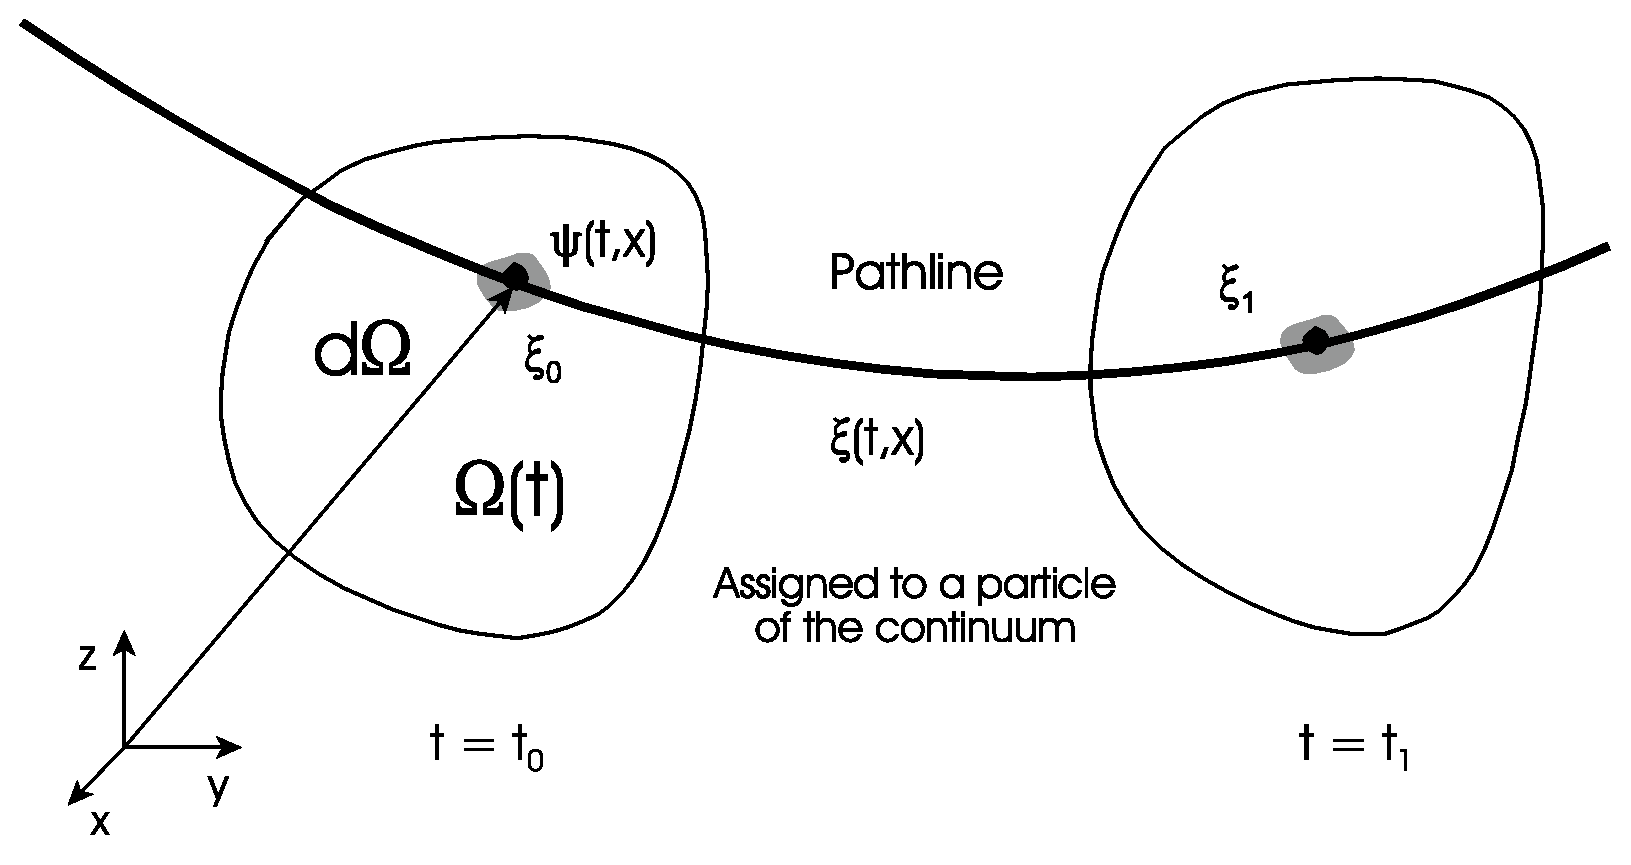
\includegraphics[width=0.8\columnwidth]{figures/mech1.eps}
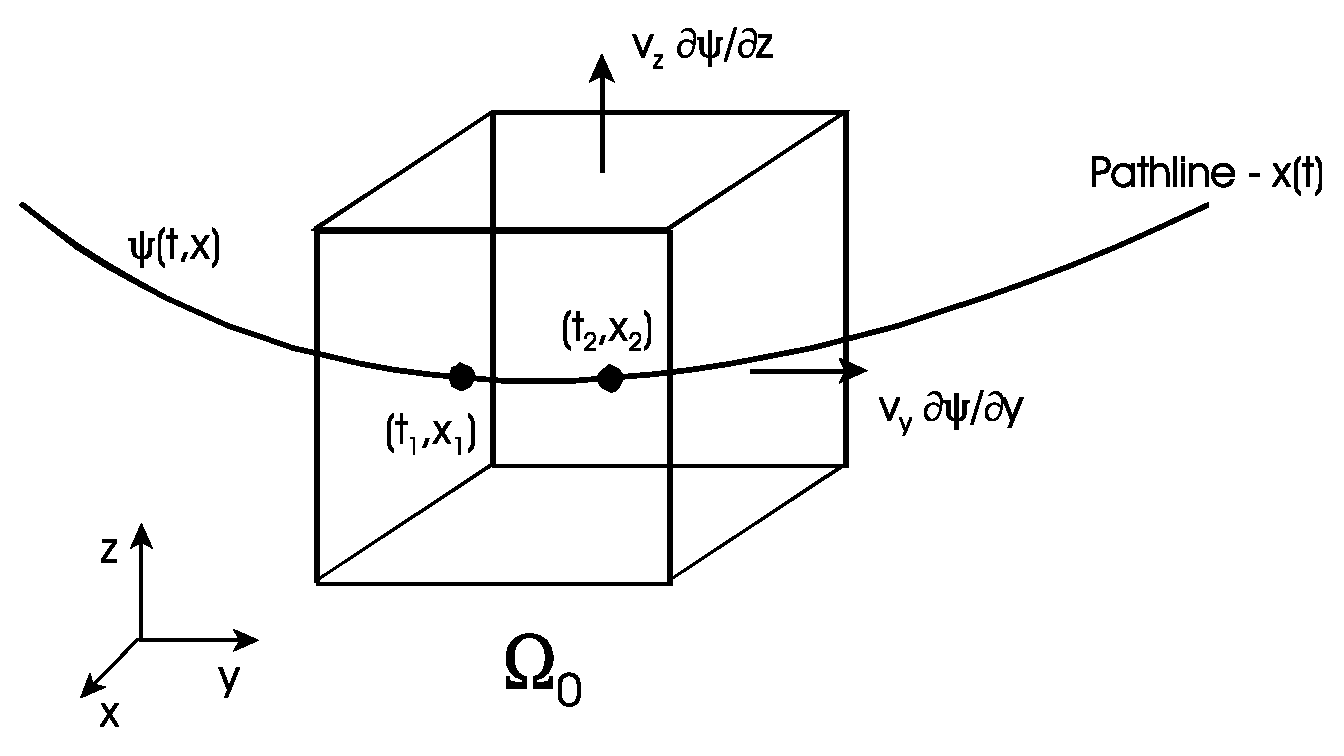
\includegraphics[width=0.8\columnwidth]{figures/mech2.eps}
\caption{Two basic descriptions of motion: Langrangian (top) and Eulerian (bottom), adopted from \cite{Kol:02}}
\label{fig:Euler-Langrange}
\end{center}
\end{figure}

The balance equations for mass, momentum and energy conservation can be derived based on two fundamental principles.
%
Both conservation principles are related by two different forms of derivatives
\begin{equation}
\frac{d \psi}{dt}
=
\frac{\p \psi}{\p t} + \v\cdot\nabla\psi
\end{equation}
the total (or material) $d$ and partial derivitives $\p$, respectively.

The general balance equation is given by
%
\begin{eqnarray}
\frac{d}{dt} \int\limits_\Omega \psi d\Omega
=
\int\limits_\Omega
\left(
\frac{\partial\psi}{\partial t}
+
\nabla \cdot {\bf J}
\right)
d\Omega
=
\int\limits_\Omega Q^\psi d\Omega
\end{eqnarray}
%
where $\psi$ is the general conservation quantity (Tab. \ref{tab:conservation_quantities}), $\bf J$ is the total flux of $\psi$, and $Q$ is a source/sink term for $\psi$.
%
The corresponding extensive and intensive conservation quantities are summarized in Tab. \ref{tab:conservation_quantities}.

%
\begin{table}[htb!]
\caption{Conservation quantities}
\label{tab:conservation_quantities}
\begin{center}
\begin{tabular}{|ll|ll|}
\hline
Extensive  quantity &  Symbol    &  Intensive quantity      &  Symbol  \\
\hline \hline
%\mbox{\rule[1mm]{0cm}{3mm}Mass}
Mass                &  $M$,$M_k$ & Mass density             & $\rho$,$\rho_k$  \\
Linear momentum     &  $\bf m$   & Linear momentum density  & $\rho \bf v$ \\
Energy              &  $E$       & Energy density           & $e = \rho i + \frac 1 2 \rho v^2 $
\\[1pt]
\hline
\end{tabular}
\end{center}
\end{table}
%

The total flux ${\bf\Phi}^\psi$ of a quantity $\psi$ is defined as
\begin{eqnarray}
{\bf\Phi}^\psi
=
{\bf v}^E \psi
\end{eqnarray}

where ${\bf v}^E$ is a mean particle velocity\index{quantity - velocity -
particle}. Physically ${\bf\Phi}^\psi$ represents the quantity of
$\psi$ passing through a unit area of the continuum, normal to
${\bf v}^E$, per unit time with respect to a fixed coordinate
system.

For the case of a multi-component continuum let ${\bf v}$ denote
the mass-weighted velocity\index{quantity - velocity - mass-weighted}
describing a more ordered motion of the particles of a fluid
element. The total flux can be written as
\begin{eqnarray}
{\bf\Phi}^\psi
=
{\bf v}^E \psi
=
\underbrace{{\bf v} \psi}_{{\bf\Phi}^\psi_A}
+
\underbrace{({\bf v}^E-{\bf v}) \psi}_{{\bf\Phi}^\psi_D}
\end{eqnarray}

and, therefore, decomposed into two parts: an advective flux
${\bf\Phi}^\psi_A$ and a diffusive flux ${\bf\Phi}^\psi_D$
relative to the mass-weighted velocity:

\begin{itemize}
 \item
$\qquad$ advective flux\index{flux - advective} of quantity $\psi$
\begin{eqnarray}
{\bf\Phi}^\psi_A
=
{\bf v}\psi
\end{eqnarray}

 \item
$\qquad$diffusive flux\index{flux - diffusive} of quantity $\psi$
(Fick's law)\index{law - Fick}
\begin{eqnarray}
{\bf\Phi}^\psi_D=
-\alpha \nabla\psi
\end{eqnarray}
\end{itemize}

This means, diffusive flux is positive in the direction of negative gradient.
